\documentclass[compress]{beamer}
\usepackage{setspace}
\usepackage{multicol}
\mode<presentation>
{
  %\usetheme{Warsaw}
  %\usecolortheme{spruce}
  % or ...
	%\useoutertheme{infolines}
  %\setbeamercovered{transparent}
  
  \usetheme{CambridgeUS}
    \setbeamercolor{item projected}{bg=darkred}
    \setbeamertemplate{enumerate items}[default]
    \setbeamertemplate{navigation symbols}{}
    \setbeamercovered{invisible}
    \setbeamercolor{block title}{fg=darkred}
    \setbeamercolor{local structure}{fg=darkred}
  
  % or whatever (possibly just delete it)
}

\usepackage{verbatim} 
\usepackage{listings}
\usepackage{tikz}
\usetikzlibrary{arrows}
\usetikzlibrary{shapes}
\tikzstyle{block}=[draw opacity=0.7,line width=1.4cm]

\newcommand{\bigpause}{\bigskip \pause}
\newcommand\azul[1]{{\color{blue}#1}}
\lstloadlanguages{C++}
\lstnewenvironment{code}
	{%\lstset{	numbers=none, frame=lines, basicstyle=\small\ttfamily, }%
	 \csname lst@SetFirstLabel\endcsname}
	{\csname lst@SaveFirstLabel\endcsname}
\lstset{% general command to set parameter(s)
	language=C++, basicstyle=\footnotesize\sffamily, keywordstyle=\slshape,
	emph=[1]{tipo,usa}, emphstyle={[1]\sffamily\bfseries},
	basewidth={0.47em,0.40em},
	columns=fixed, fontadjust, resetmargins, xrightmargin=5pt, xleftmargin=15pt,
	flexiblecolumns=false, tabsize=2, breaklines,	breakatwhitespace=false, extendedchars=true,
	numbers=left, numberstyle=\tiny, stepnumber=1, numbersep=9pt,
	frame=l, framesep=3pt,
}

\usepackage[spanish]{babel}
% or whatever

\usepackage[utf8]{inputenc}
% or whatever

\usepackage{times}
\usepackage[T1]{fontenc}
% Or whatever. Note that the encoding and the font should match. If T1
% does not look nice, try deleting the line with the fontenc.


\title[Topological Sort y SCC] % (optional, use only with long paper titles)
{Topological Sort y Componentes Fuertemente Conexas}

\author[Melanie Sclar] % (optional, use only with lots of authors)
{~Melanie Sclar}
% - Give the names in the same order as the appear in the paper.
% - Use the \inst{?} command only if the authors have different
%   affiliation.
\institute[UBA] % (optional, but mostly needed)
{
  %\inst{1}%
  Facultad de Ciencias Exactas y Naturales\\
  Universidad de Buenos Aires
}
\date[PAP] % (optional, should be abbreviation of conference name)
{Problemas, Algoritmos y Programación}

% Delete this, if you do not want the table of contents to pop up at
% the beginning of each subsection:
\AtBeginSubsection[]
{
  \begin{frame}<beamer>{Contenidos}
    \tableofcontents[currentsection,currentsubsection]
  \end{frame}
}

%\newcommand{\be}{\begin{equation*}}
\newcommand{\ee}{\end{equation*}}
\newcommand{\state}[1]{\left|\,#1\,\right\rangle}
\newcommand{\costate}[1]{\left\langle\,#1\,\right|}
\newcommand{\trace}{\text{Tr}}
\newcommand{\su}{\uparrow}
\newcommand{\sd}{\downarrow}
\newcommand{\im}{\text{Im}}
\newcommand{\re}{\text{Re}}

% If you wish to uncover everything in a step-wise fashion, uncomment
% the following command:

%\beamerdefaultoverlayspecification{<+->}


\begin{document}
\pgfdeclarelayer{background}
\pgfsetlayers{background,main}
\begin{frame}
  \titlepage
\end{frame}

\section{Topological Sort}
\subsection{Motivación}
\begin{frame}{Grafos hasta para vestirse}
Muchas veces \textbf{tenemos un orden parcial que nos gustaría extender a un orden
total}. Por ejemplo si construyéramos un grafo de precedencia para vestirnos, sabemos que: \\
\bigskip

medias $\rightarrow$ zapatillas \\
ropa interior $\rightarrow$ pantalón \\
pantalón $\rightarrow$ zapatillas \\

\bigskip

Pero esto aún nos deja libertad respecto del orden total final, 
pues tenemos estos dos órdenes totales: \\
\bigskip

medias $\rightarrow$ ropa interior $\rightarrow$ pantalón $\rightarrow$ zapatillas \\
ropa interior $\rightarrow$ medias $\rightarrow$ pantalón $\rightarrow$ zapatillas

\end{frame}

\begin{frame}

Este no es el único ejemplo: siempre que tengamos muchas tareas a realizar
con algunas precedencias preestablecidas y debamos definir el orden total
en el que las mismas se realizarán (no podemos paralelizarlas), será útil
lo que veremos hoy. \\

\bigskip

\begin{block}{Topological Sort}
Un \textit{topological sort} de un DAG (Directed Acyclic Graph) $G$ 
es un ordenamiento de todos sus nodos de manera tal que si $G$ contiene
un eje $(u, v)$, entonces $u$ aparece antes que $v$ en el ordenamiento.
\end{block}

\end{frame}

\subsection{Topological Sort con in-degree}
\begin{frame}{Topological sort con in-degree}

Existen varias formas de resolver este problema. La que más me gusta
observa que cada nodo tiene un $in-degree$ particular.

\begin{block}{in-degree de un nodo}
Se define el $in-degree$ de un nodo $v \in V(G)$ como la cantidad de
ejes incidentes en $v$ en el grafo $G$. Lo notamos $in[v]$.
\end{block}

\begin{itemize}
\item Cuando $in[v] = 0$, $v$ no tiene ninguna dependencia que le impida ir
en este momento en el ordenamiento total. 
\item Al agregar $v$ al ordenamiento
total, esto modifica el $in-degree$ de todos los $w$ tal que existe $(v,w) \in E(G)$.
\end{itemize}

\end{frame}

\begin{frame}{Topological sort con in-degree}

\begin{itemize}
\item Con estas observaciones, podemos ver que si en cada momento elegimos un
nodo con $indegree$ igual a 0 y lo colocamos como próximo nodo del ordenamiento,
cuando hagamos esto sobre todos los nodos tendremos un topological sort.
Es importante recordar actualizar el $indegree$ de los vecinos.

\item Cuando hay varios candidatos posibles, podemos elegir cualquiera de ellos.
En general, todos los candidatos se guardan en una cola, pero esto dependerá 
del problema que estemos resolviendo.

\item Si en algún momento no tenemos más nodos con $indegree = 0$ pero aún no
colocamos todos los nodos, significa que el grafo no era un DAG.
\end{itemize}

\end{frame}


\begin{frame}[fragile]{Pseudocódigo del toposort con in-degree}

\begin{lstlisting}
L = Lista vacia que contendra los elementos ordenados
S = Conjunto de nodos sin nodos entrantes (in-degree = 0)

mientras S no sea vacio:
    removemos un nodo v de S (cualquiera sirve)
    agregamos v al final de L
    para cada nodo w tal que existe el eje (v, w):
        removemos (v, w) del grafo (indegree[w] = indegree[w] - 1)
        si no hay mas ejes incidentes en w (indegree[w] == 0):
            insertar w en S
            
si el grafo aun tiene ejes retorno error (no era DAG)
si no, retorno L
\end{lstlisting}

Se puede ver que la complejidad será $O(n+m)$.
\end{frame}

\subsection{Topological Sort con DFS}
\begin{frame}{Topological Sort con DFS}

Utilizando la notación de la clase pasada, recorremos el grafo con DFS
colocando dos números en cada nodo: el tiempo de descubrimiento y el de
finalización. \\
\bigskip

A medida que vayamos finalizando cada nodo, lo iremos agregando al frente
de la lista del orden topológico. Así, el que termina último deberá ir
primero en el orden final (lo que es intuitivo, porque de él dependen
muchos de los otros nodos).
\end{frame}

\begin{frame}{Ejemplo de Topological Sort con DFS}
\begin{center}
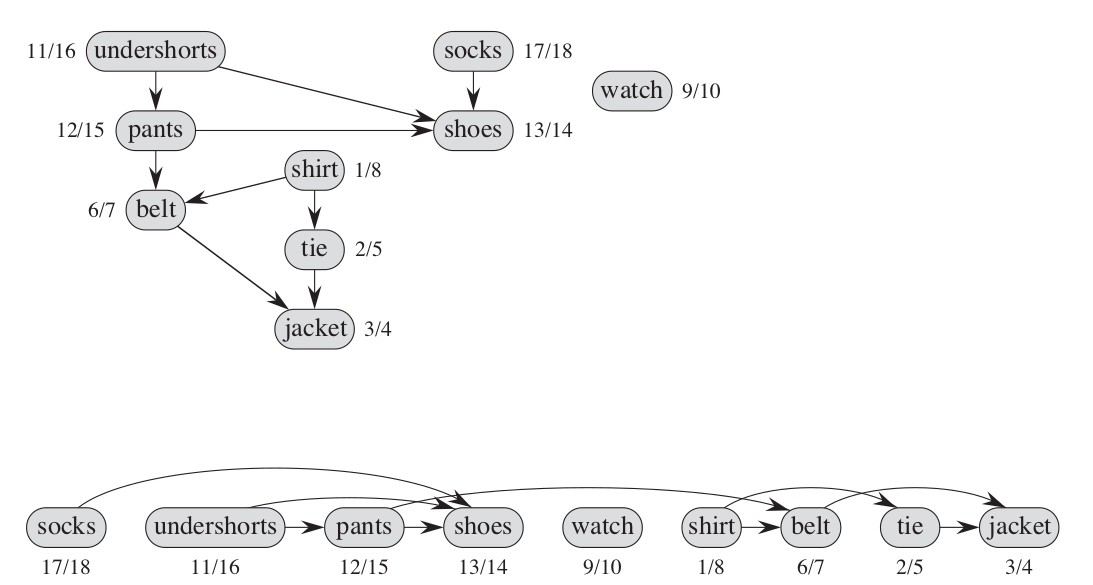
\includegraphics[width=0.9\linewidth]{toposort-dfs.png}
\end{center}

\begin{flushright}
\tiny Ejemplo totalmente no robado del Cormen
\end{flushright}

\end{frame}

\begin{frame}{Pseudocódigo de Topological Sort con DFS}

\begin{enumerate}
\item Correr DFS sobre $G$ para computar los tiempos de finalización de cada nodo
\item A medida que cada vértice sea finalizado, lo inserto en el frente de la lista de respuesta
\item Devuelvo la lista, que representa un topological sort de G
\end{enumerate}

La complejidad será $O(n+m)$, pues sólo consiste en correr un DFS.

\end{frame}

\begin{frame}{Correctitud de Topological Sort con DFS}

\begin{block}{Un DAG no contiene back edges}
Un grafo $G$ dirigido es acíclico si y sólo si un DFS de $G$ no tiene
$back$ $edges$. Recordemos que una back edge es un eje $(u, v)$ que conecta
a $u$ con $v$, un antecesor de $u$ en el árbol de DFS.
\end{block}
\bigpause

Idea de la demo: si tuviera un back edge, ese formaría un ciclo.

\bigpause

Debemos ver que para todo $(u, v) \in E(G)$, vale que $v.f < u.f$. Si vemos
esto entonces podemos observar que al momento de agregar un nodo al frente 
de lista respuesta todos los ejes incidentes en él tienen finishing 
time posterior. Esto implica que los ejes estarán bien ordenados en el toposort.

\end{frame}

\begin{frame}{Correctitud de Topological Sort con DFS (2)}

Por suerte, es fácil ver que para todo $(u, v) \in E(G)$, vale que $v.f < u.f$:

\bigskip

Si al momento de recorrer $(u,v)$ ya tuviéramos a $v$ marcado de gris (es decir,
ya tiene tiempo inicial pero no final) entonces $v$ sería ancestro de $u$ y $(u,v)$
sería un back edge. ¡Absurdo!

\bigskip
Entonces $v$ es o bien blanco o negro (nunca tocado, o ya finalizado).
\begin{itemize}
\item Si $v$ fuera blanco, $v$ es descendiente de $u$ y luego $v.f < u.f$
\item Si $v$ fuera negro, $v$ ya se terminó y por lo tanto $v.f$ ya está
definido. Pero $u.f$ todavía no está definido, y luego sabemos que $v.f < u.f$.
\end{itemize}

\end{frame}

\subsection{Problemas}
\begin{frame}{Problema: conservación de la Mona Lisa}

{ \scriptsize
La Mona Lisa debe ser conservada: este trabajo será realizado en dos
laboratorios especializados en distintas tareas. El proceso de 
conservación se ha dividido en varias etapas y para cada una de ellas 
sabemos en qué laboratorio deberá realizarse.
\bigskip

Transportar la tan famosa pintura introduce un riesgo adicional, por lo
que debemos evitarlo siempre que sea posible. Idealmente, primero se
realizarían todos los trabajos en el primer laboratorio para luego mover
la pintura para el segundo laboratorio y completar las tareas.
\bigskip

Sin embargo, hay numerosas dependencias entre etapas de conservación -
algunas deben completarse antes que otras puedan comenzar. Debemos
encontrar un orden para realizar las tareas tal que se minimice el
número de veces que la pintura necesita ser movida entre laboratorios.
La conservación puede comenzar en cualquier laboratorio.
\bigskip

\# tareas $\leq$ 100000, \# dependencias $\leq$ 1000000
\bigskip

\texttt{https://icpcarchive.ecs.baylor.edu/index.php?
option=com\_onlinejudge\&Itemid=8\&category=567\&page=
show\_problem\&problem=4275}

}
\end{frame}

\begin{frame}{Solución: conservación de la Mona Lisa}

\begin{itemize}
\item Básicamente, queremos un topological sort de las tareas pero 
siempre que sea posible tomaremos una tarea del mismo laboratorio donde
nos encontramos actualmente.
\item Cuando esto no sea posible, ahí tomaremos una tarea del otro
laboratorio, contabilizando este cambio.
\item Como no sabemos en qué laboratorio comenzamos, probamos ambos
posibles comienzos y tomamos el que menos cambios entre laboratorios
produzca.
\end{itemize}

\end{frame}

\begin{frame}{Combinando Topological Sort con otras técnicas}

\begin{itemize}
\item Muchas veces el topological sort (o $toposort$, para los amigos) no
soluciona completamente el problema, pero es un paso necesario en el
camino a la solución.

\item Por ejemplo, a partir de llevar al grafo a un orden topológico 
podemos utilizar técnicas que requieren de la noción de $anterior$,
como programación dinámica (entre muchas otras).
\end{itemize}

\end{frame}


\begin{frame}{Problema: camino máximo en un DAG}

Dado un DAG con pesos, queremos hallar un camino máximo en él. Es decir,
entre todos los caminos posibles, queremos hallar uno cuya suma de los
ejes sea máxima.

\bigskip

Veamos un ejemplo en el pizarrón.

\bigskip

\begin{center}
\textquestiondown Ideas?
\end{center}

\end{frame}

\begin{frame}{Solución: camino máximo en un DAG}

Este problema es esencialmente programación dinámica, pero no podríamos
aplicarla sin dar un orden para los nodos. Sin un orden adecuado,
\textquestiondown cuál sería el caso recursivo? \textquestiondown
cómo sé que es más pequeño?

\bigskip

Tomo un topological sort de $G$, que denotaré $ordenTopologico(G)$.

Si estoy en $w$, todos los ejes que llegan a $w$ partieron de un nodo
anterior según $ordenTopologico(G)$. Así, para cada uno de ellos puedo
asumir que la distancia máxima ya está calculada y fijarme si al agregar
el costo de la arista obtengo un nuevo camino máximo terminando en $w$
o no. \\

\end{frame}

\begin{frame}[fragile]{Solución: camino máximo en un DAG}

\begin{lstlisting}
para cada vertice v en ordenTopologico(G):
    para cada eje (v, w) en E(G):
        distancia[w] = max(distancia[w], distancia[v] + peso (G, (v, w)))

devolver maxima distancia[v] entre todos los v en V(G)
\end{lstlisting}

\bigskip

\textquestiondown A qué problema clásico de programación dinámica les
suena este problema?

\end{frame}

\section{Componentes fuertemente conexas}
\subsection{Motivación}
\begin{frame}{Componentes fuertemente conexas}

En grafos no dirigidos ya vimos la noción de componentes conexas: son
subgrafos conexos maximales, es decir, subgrafos conexos donde al agregar
un nodo más (si existiera alguno) el subgrafo dejaría de ser conexo. \\

\bigskip

En el párrafo anterior, un grafo conexo es un grafo donde entre existe
un camino entre cualquier par de nodos que lo forman. \\

\bigskip

\textquestiondown Cómo podemos extender esto a grafos dirigidos? Aquí
no siempre que desde $A$ podemos llegar a $B$ significa que desde $B$
podemos llegar a $A$. Veamos un ejemplo en el pizarrón.

\end{frame}


\begin{frame}{Componentes fuertemente conexas}

\begin{block}{Grafo fuertemente conexo}
Un grafo fuertemente conexo es un grafo $G$ dirigido en el cual para
todo par de nodos $v$, $w$ ($v \neq w$) existe un camino que parte de $v$
y llega a $w$ y viceversa.
\end{block}

\bigskip

La mayoría de los grafos no son fuertemente conexos, pero podemos
separar los nodos en subgrafos tal que cada uno lo sea.

\end{frame}

\begin{frame}{Ejemplo visual}

Dibujar ejemplo en el pizarrón donde marco las componentes fuertemente 
conexas. Usá tu creatividad.

\end{frame}

\begin{frame}{Checkear si un grafo es fuertemente conexo}
Primero resolvamos una versión más sencilla del problema que queremos
resolver. Supongamos que sólo nos interesara saber si un grafo es fuertemente
conexo o no. \textquestiondown Qué podemos hacer?

\bigpause

Podemos partir de un nodo cualquiera $u$ y hacer DFS desde $u$. Si no
pude llegar a todos los nodos, no era fuertemente conexo (\textquestiondown por qué?).
Si pude, entonces invierto la dirección de todos los ejes de $G$ y hago
DFS desde $u$ nuevamente. Si de nuevo pude llegar a todos los nodos,
significa que en el grafo original puedo llegar desde cualquier nodo a $u$.

\begin{center}
$u \leadsto v$ y $v \leadsto u$ para todo $v \in V(G)$
\end{center}

Luego, es un grafo fuertemente conexo.

\end{frame}


\subsection{Algoritmo de Kosaraju}
\begin{frame}{Algoritmo de Kosaraju}

\begin{enumerate}
\item Correr $DFS(G)$ computando los tiempos de finalización $u.f$ para cada nodo $u \in V(G)$
\item Calcular $G^T$
\item Correr $DFS(G^T)$, pero en el ciclo central del DFS consideramos
los vértices en orden decreciente según el tiempo de finalización calculado
en el ítem 1.
\item Imprimir los vértices de cada árbol del bosque de DFS formado en la línea
3 como una componente fuertemente conexa.
\end{enumerate}
\end{frame}

\begin{frame}
Corramos un ejemplo en el pizarrón para ganar intuición de por qué funciona
el algoritmo. Luego, pensemos por qué funciona!

\bigskip
Nota: el ejemplo hecho a mano se adjunta en \texttt{kosaraju.jpg}
\end{frame}

\begin{frame}
\begin{center}
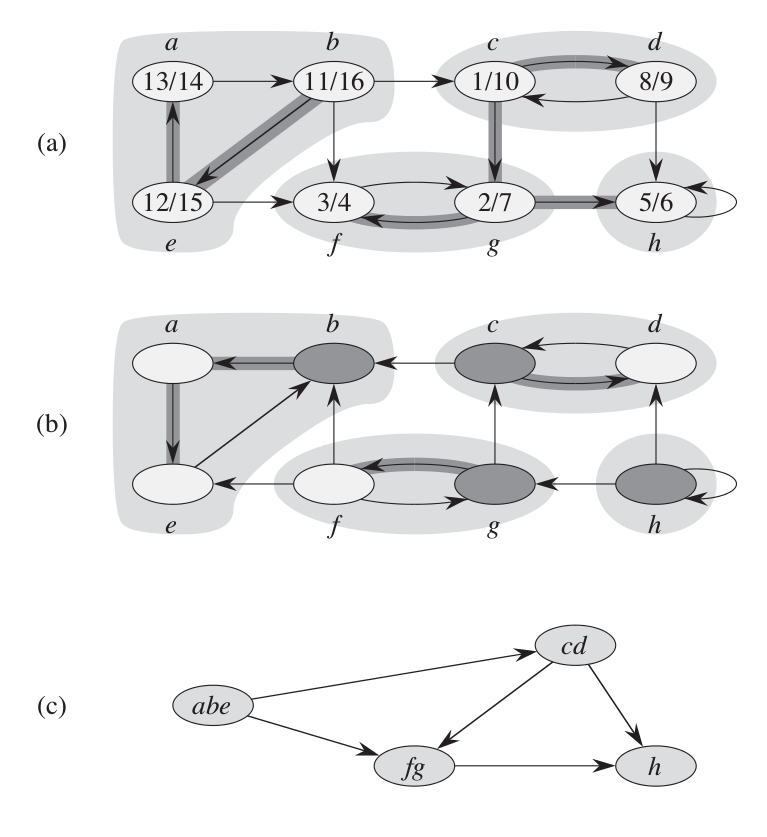
\includegraphics[width=0.5\linewidth]{kosaraju.png}
\end{center}
\end{frame}

\begin{frame}{Demo de Kosaraju: observaciones}
\begin{itemize}
\item Una vez que separo el grafo en componentes fuertemente conexas,
si pienso a cada componente como un nodo (les voy a decir 
``supernodos''), dicho grafo es un DAG. Esto es así porque si contuviera un ciclo, 
todos los supernodos formarían parte de una misma componente fuertemente
conexa, lo que sería absurdo.
\item $G$ y $G^T$ tienen las mismas componentes fuertemente conexas ($G^T$
es $G$ transpuesto, o sea, todos los ejes invierten su dirección).
\end{itemize}
\end{frame}

\begin{frame}{Demo de Kosaraju}
Veremos por inducción que cada árbol del $DFS(G^T)$ se corresponde con una
componente fuertemente conexa de $G$ (o $G^T$, pues son las mismas).
\bigskip
Supongamos que los primeros $k$ árboles explorados en $DFS(G^T)$ son
componentes fuertemente conexas (SCC para abreviar). Veamos que el $k+1$-ésimo
lo será (el caso base con $k = 0$ es trivial).
\end{frame}

\begin{frame}{Demo de Kosaraju}
Como elijo las raíces del $DFS(G^T)$ en orden descendiente de 
finishing time, sé que los tiempos de las raíces de los árboles 
todavía no visitados son menores al que voy a analizar ahora.

\bigskip
Más aún, definamos $f(C) = $ máximo finishing time de la componente $C$.

\bigskip
Sea $u$ es la raíz del árbol que estamos analizando, y $u \in C$ (C es SCC).
Entonces $u.f = f(C) > f(C')$ para todo $C'$ componente conexa aún no hallada
(por como elegimos las raíces del DFS).
\end{frame}


\begin{frame}{Demo de Kosaraju (2)}
\begin{block}{Lema que me van a creer}
Sea $G = (V, E)$, $(u, v) \in E$, y sean $C, C'$ SCC's tal que $u \in C$
y $v \in C'$. Entonces, $f(C) > f(C')$.
\end{block}

\begin{block}{Corolario del lema que me creyeron}
Sea $G = (V, E)$, $(u, v) \in E^T$, y sean $C, C'$ SCC's tal que $u \in C$
y $v \in C'$. Entonces, $f(C) < f(C')$.
\end{block}
\end{frame}

\begin{frame}{Demo de Kosaraju (3)}
Así, todos los ejes que ``salen'' del árbol que estamos explorando van para
componentes anteriores, que ya fueron analizados. ¿Por qué?

\bigpause

¡Por el corolario anterior! Si hay un eje $(u,v) \in E^T$ con $u \in C$,
luego $f(C) < f(C')$ siendo $v \in C'$. Pero ya comentamos que los árboles
que vienen después tienen finishing times menores por como es nuestro algoritmo,
luego los únicos que cumplen con $f(C) < f(C')$ son los $C'$ ANTERIORES a $C$.
\end{frame}

\begin{frame}{Demo de Kosaraju (4 - gran final)}
{Conclusiones maravillosas}

\begin{itemize}
\item Todos los nodos de $C$ se visitan al explorar el árbol de DFS enraizado 
en $u$ (si no, significa que en $G$ no vale que $v \leadsto u$, una de las
condiciones de SCC).
\item En la exploración del árbol de DFS que comienza en $u$, no se visitan
nodos que no pertenezcan a la SCC: todos los vértices que puedo alcanzar son
o bien pertenecientes a $C$ o son de componentes anteriores, que ya terminé de
explorar por hipótesis inductiva (y son de otra SCC).
\end{itemize}

Entonces, como no faltan ni sobran nodos, el $k+1$-ésimo árbol es una SCC de $G$!

\end{frame}

\subsection{Problemas}
\begin{frame}{Componentes semiconexas}
Un grafo dirigido $G$ es semiconexo si para todo par de vértices $u, v \in V(G)$
vale que o bien $u \leadsto v$ o bien $v \leadsto u$. Dar un algoritmo
eficiente para determinar si $G$ es semiconexo o no.
\end{frame}

\begin{frame}{Solución: Componentes semiconexas}
\begin{itemize}
\item Separo $G$ en componentes fuertemente conexas. Lo que me queda es un DAG.
\textquestiondown Cómo debe ser este DAG para que se cumpla la propiedad de
semiconexión?
\bigpause
\item  Básicamente, debe ser un DAG que tenga un único topological sort.
\bigpause
\item  O dicho de otra forma, un grafo palito con posibles aristas agregadas (pensar por qué).
\end{itemize}
\end{frame}

\begin{frame}{Idea para ver por qué el DAG debe ser único}
\begin{itemize}
\item Si hubiera 2 o más nodos a los cuales sólo inciden ejes (no salen
ejes desde ellos) entonces no será semiconexo (no tengo cómo deducir
uno de estos nodos del otro).
\item Si hubiera 0 nodos a los cuales sólo inciden ejes, no era un DAG
sobre lo que partimos. Sabemos que lo es pues el grafo que queda luego
de las componentes fuertemente conexas.
\item Entonces hay exactamente un nodo al cual sólo le inciden ejes. Ese 
es claramente el último del topological sort. Lo quito y aplico el mismo
principio recursivamente.
\end{itemize}
\end{frame}


\begin{frame}{Problema: 2-SAT con SCC}

Queremos resolver 2-SAT utilizando componentes fuertemente conexas.
Esto nos permitirá tener una solución lineal. Recordemos 2-SAT: \\

\bigskip

\begin{block}{2-SAT}
El problema de 2-SAT consiste en determinar si a una colección de 
variables con dos valores posibles y restricciones entre pares de 
variables se le puede asignar un valor satisfaciendo todas las 
restricciones.
\end{block}

\bigskip

Veamos un ejemplo.

\end{frame}

\begin{frame}

Esta podría ser una posible entrada para el problema. Cada variable
puede tener dos valores posibles, que de ahora en más llamaremos $True$
y $False$, y queremos que toda la expresión sea verdadera. \\
\bigskip

$$(x_0\lor x_2)\land(x_0\lor\lnot x_3)\land(x_1\lor\lnot x_3)\land(x_1\lor\lnot x_4)\land$$
$$(x_2\lor\lnot x_4)\land{}(x_0\lor \lnot x_5)\land (x_1\lor\lnot x_5)\land (x_2\lor\lnot x_5)\land$$
$$(x_3\lor x_6)\land (x_4\lor x_6)\land (x_5\lor x_6)$$

\bigskip

Nos gustaría poder modelar las restricciones con un grafo. 
\textquestiondown Ideas?

\end{frame}

\begin{frame}{2-SAT: modelado del grafo}
\begin{itemize}
\item Podemos pensar que un eje dirigido $(u,v)$ significa que $u$ implica $v$.

\item Modelamos los nodos como cada variable y su negación: tendremos un nodo
$x_i$ y otro nodo $\lnot x_i$ para todo $i$.

\item \textquestiondown Cómo deben ser los ejes que modelen las fórmulas
binarias de la entrada?
\end{itemize}

\bigpause
\begin{center}
$a \lor b \ \ \ \equiv \ \ \ \lnot a \rightarrow b \ \ \ \equiv \ \ \ a \rightarrow \lnot b$
\end{center}

\end{frame}

\begin{frame}

$$(x_0\lor x_2)\land(x_0\lor\lnot x_3)\land(x_1\lor\lnot x_3)\land(x_1\lor\lnot x_4)\land$$
$$(x_2\lor\lnot x_4)\land{}(x_0\lor \lnot x_5)\land (x_1\lor\lnot x_5)\land (x_2\lor\lnot x_5)\land$$
$$(x_3\lor x_6)\land (x_4\lor x_6)\land (x_5\lor x_6)$$

\bigskip

\begin{center}
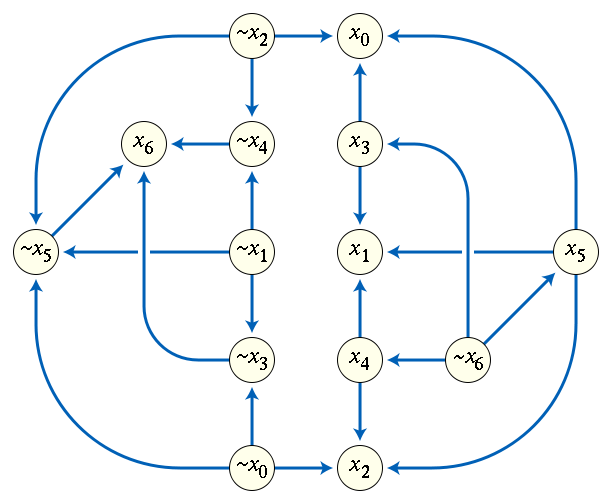
\includegraphics[height=5cm]{2sat.png}
\end{center}

\end{frame}

\begin{frame}{2-SAT: observaciones clave}
\begin{itemize}
\item La fórmula es insatisfactible si y sólo si $x_i$ implica $\lnot x_i$
y viceversa. \textquestiondown Por qué no alcanza sólo uno de los dos?
\item Pensando en nuestro modelado con grafos, esto significa que
la fórmula es insatisfactible si $x_i$ y $\lnot x_i$ están en la misma
componente fuertemente conexa (existe un camino de implicaciones que parte
de uno y llega al otro para ambos).
\end{itemize}
\end{frame}

\begin{frame}{Solución 2-SAT (existencia)}
\begin{itemize}
\item Así, corriendo Kosaraju detecto las componentes fuertemente conexas
y checkeo que no haya ningún $x_i$ y $\lnot x_i$ en la misma componente.
\item Supongamos que no hay, entonces existe una asignación de valores
a los $x_i$ que resuelve el problema. \textquestiondown Pero cómo hallo 
dicha asignación?
\end{itemize}
\end{frame}

\begin{frame}{Solución 2-SAT (construcción de la respuesta)}

Notemos que si una componente conexa contiene los elementos 
$a_1, a_2, ..., a_k$ entonces existe otra que contiene la negación 
de todos estos: $\lnot a_1, \lnot a_2, ..., \lnot a_k$. \\

\bigskip 
Esto es así porque si $a_1 \rightarrow a_2$ es equivalente a su
contrarrecíproco $\lnot a_2 \rightarrow \lnot a_1$ y el grafo de 2-SAT
contiene todas las implicaciones entre elementos.

\bigskip

Entonces tenemos un DAG de las componentes fuertemente conexas: por ser
DAG, qué podemos hacer con sus nodos? \pause ¡Un topological sort!

\end{frame}

\begin{frame}
\begin{itemize}
\item Notemos que podemos pensar que cada componente fuertemente conexa 
tiene una pareja, que es aquella con los mismos elementos pero negados.
\item Si $C_1$ y $C_2$ son pareja, entonces $u \in C_1 \leadsto \lnot u \in C_2$ o
viceversa, pues $x \leadsto \lnot x \lor \lnot x \leadsto x$ siempre
es cierto.
\item Así, tomamos un topological sort y lo empezamos a analizar en
orden inverso. Si la componente $C_i$ no tenía valores asignados, coloco
todos sus nodos en $True$. Como consecuencia, todos los de la pareja de $C_i$
(que tiene todos los mismos elementos pero negados) irán en $False$.
\item Notemos que esto no generará implicaciones del estilo $True \rightarrow False$,
que son las que queremos evitar, pues tomamos el toposort en orden inverso.
\end{itemize}
\end{frame}

\begin{frame}
\begin{center}
{\Huge \textquestiondown Preguntas?}
\end{center}
\end{frame}

\end{document}

\section*{Bibliograf\'ia}

\subsection*{Bibliograf\'ia}

\begin{frame}{Bibliograf\'ia}
\begin{itemize}
\item \textit{Introduction to Algorithms, 2nd Edition}. MIT Press. \\ Thomas H. Cormen \\ Charles E. Leiserson \\ Ronald L. Rivest \\ Clifford Stein \\
Secci\'on 22 (Elementary Graph Algorithms)
\item Micha Sharir. A strong connectivity algorithm and its applications to data flow analysis. Computers and Mathematics with Applications 7(1):67–72, 1981.(\azul{\href{http://www.sciencedirect.com/science/article/pii/0898122181900080}{Link}})
\item Tarjan, R. Depth first search and linear graph algorithms. SIAM J Comput. 1972;1:146–160.(\azul{\href{http://epubs.siam.org/doi/abs/10.1137/0201010}{Link}})
\end{itemize}

\end{frame}


\end{document}
